% Chapter 1

\chapter{Progetto Aziendale} % Main chapter title

\label{Chapter2} % For referencing the chapter elsewhere, use \ref{Chapter1} 

\lhead{Capitolo 2. \emph{Progetto Aziendale}} % This is for the header on each page - perhaps a shortened title

%----------------------------------------------------------------------------------------
Come annunciato nel precedente capitolo, cardini di questo progetto sono il rilevamento del volto (e delle sue parti) e la condivisione di contenuti attraverso i Social Networks.
A seguire verranno fornite informazioni di carattere formativo su tali punti.

\section{Rilevamento facciale}

Il rilevamento facciale è una tecnica di intelligenza artificiale utilizzata per verificare la presenza di un volto a partire da una o più immagini che lo ritraggono.\\
Si può affermare che si tratti di un riconoscimento di pattern (dove il pattern da riconoscere è un volto umano), che avviene mediante tecniche di elaborazione di immagini digitali. Viene utilizzato in biometria, per sistemi di videosorveglianza ma anche per usi generici, come ad esempio per l'autofocus nelle odierne fotocamere digitali. 

Negli anni sono stati creati numerosi algoritmi a tale scopo.
Alcuni di essi usano analizzano:

\begin{itemize}
\item il colore della pelle (nelle immagini a colori)
\item il movimento (nei video)
\item la forma della testa
\item combinazione delle caratteristiche sopra elencate
\end{itemize}

Comunque si scelga l'algoritmo, le problematiche che si incontrano nella ricerca della presenza di volti sono:

\begin{itemize}
\item Qualità dell'immagine non adeguata (sgranata, non a fuoco, risoluzione insufficiente)
\item Condizione d'illuminazione non ottimale (sottoesposizione o sovraesposizione eccessiva)
\item Espressioni facciali non campionate (quando i volti presenti assumono espressioni non presenti nel template di confronto)
\item Variazione della "messa in posa"
\item Variazioni dei lineamenti del volto (ad esempio i tratti di un volto di una persona di origine asiatica saranno notevolmente diversi da quelli di una persona di origine europea)
\item Variazione di espressioni facciali
\end{itemize}

\subsection{Machine Learning}

Data la complessità del problema è difficile creare una soluzione unica che abbia un'accuratezza soddisfacente. Una delle strade migliori è costruire un classificatore e collezionare una grande database di esempi di classificazione, creare una funzione di classificazione parametrizzata e successivamente ottimizzarla. Questa metodologia è definita machine learning. 

Ne è un esempio la tecnica di rilevamento facciale sviluppato da Paul Viola e Michael Jones che utilizza le cosiddette \textit{diagonal features} all'interno di un classificatore chiamato \textit{Haar}. Questo classificatore utilizza un algoritmo di tipo \textbf{\textit{AdaBoost}} (Adaptive Boosting) ma lo organizza come una cascata di nodi dove ogni nodo è un un multi albero di classificatori AdaBoost istruiti per avere un altissimo rate di rilevamento. Tale "istruzione" deriva dal training dato dalle Haar-like features ricavate da immagini digitali. Queste immagini contengono volti normalizzati (scalati e traslati) correttamente per un rapporto 1:6000 rispetto al totale delle immagini utilizzate (le rimanenti non rappresentano facce).


\begin{figure}[H]\centering  
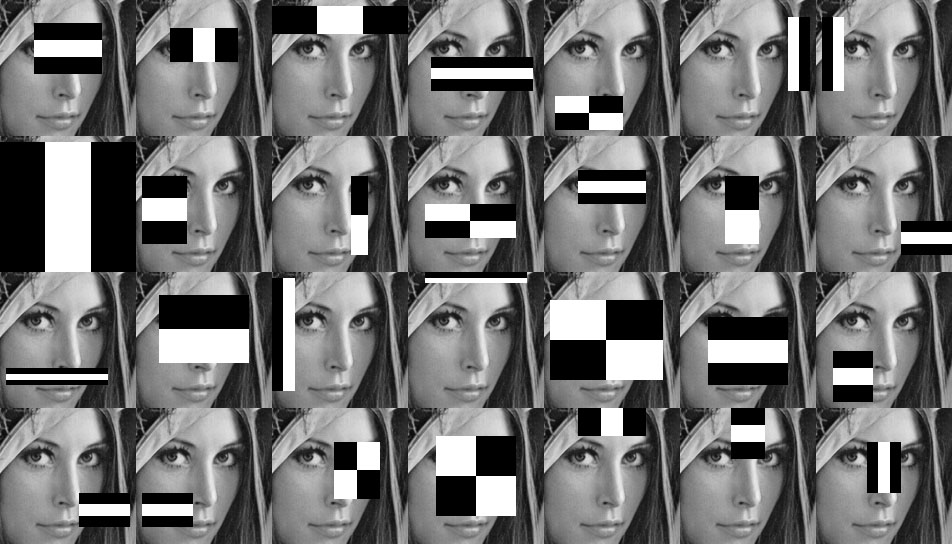
\includegraphics[scale=0.32]{/workspace/1911_up/Dropbox/thesis/Figures/feature.jpg}
\caption[Esempio di utilizzo delle features]{Esempio di utilizzo delle features}
\label{pic-a}
\end{figure}

Ad ogni nodo raggiunto, un singolo risultato negativo porta alla terminazione del processo, e l'algoritmo esce dichiarando di non aver trovato volti all'interno dell'immagine data. Ogni nodo deve rispondere nella seguente forma: 

Il valore \textit{k} trovato per la feature \textit{f} è sotto o sopra a una certa soglia \textit{S}? 
\begin{itemize}
\item \textbf{Si}, quindi la regione di interesse considerata è un volto.
\item \textbf{No}, altrimenti.
\end{itemize}

Tipicamente i nodi sono ordinati dal meno al più complesso (i primi nodi sono generalmente molto semplici). In tal modo si può ridurre notevolmente il costo computazionale di rilevamento del volto, perché le regioni dell'immagine che non lo contengono terminano subito nei primissimi nodi se non al primo.

\begin{figure}[H]\centering  
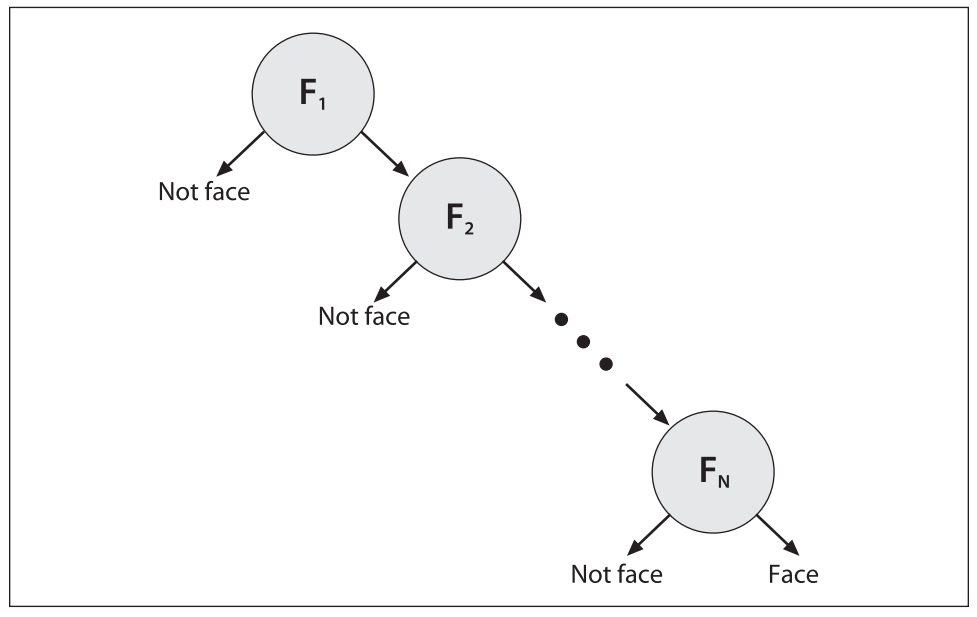
\includegraphics[scale=0.27]{/workspace/1911_up/Dropbox/thesis/Figures/boosted.png}
\caption[Binary Rejection cascade]{Binary Rejection cascade}
\label{pic-a}
\end{figure}

Tale algoritmo permette di raggiungere un alto tasso di accuratezza, infatti in media il numero di falsi negativi è inferiore all' 1 per cento mentre il numero di falsi positivi si attesta sotto al 40 per cento.

A seguire un esempio .xml di una possibile struttura di classificatore Haar:
\begin{lstlisting}
  <stages>
    <_>
      <!-- stage 0 -->
      <trees>
        <_>
          <!-- tree 0 -->
          <_>
            <!-- root node -->
            <feature>
              <rects>
                <_>
                  0 0 14 9 -1.</_>
                <_>
                  0 3 14 3 3.</_></rects>
              <tilted>0</tilted></feature>
            <threshold>-0.1192855015397072</threshold>
            <left_val>0.7854182124137878</left_val>
            <right_val>-0.4541360139846802</right_val></_></_>
        <_>
          <!-- tree 1 -->
			.
\end{lstlisting}
\section{Condivisione Social}

I siti di reti sociali (social network sites) sono servizi web che tipicamente permettono di:
\begin{itemize}
\item Creare un profilo pubblico o semi-pubblico all'interno di un sistema vincolato
\item Ottenere una lista di contatti associata a tale profilo
\item Condividere sul proprio profilo o su quello altrui contenuti testuali o multimediali
\end{itemize}

Una relazione sociale costruita sulla base di un interesse è totalmente differente da una costruita a partire da reti sociali virtuali, in cui il legame nasce a prescindere dalla presenza di interessi comuni o informazioni da condividere.
L'idea alla base di quest'ultima rete è che ogni utente possa avere uno scambio bidirezionale di informazioni con altri utenti. In un'era in cui buona parte della popolazione mondiale utilizza tale strumento di comunicazione, è quindi spesso fondamentale integrare al software funzionalità di condivisione.

\begin{figure}[H]\centering  
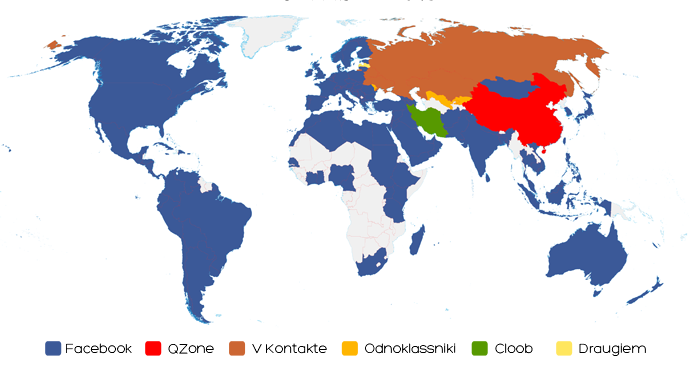
\includegraphics[scale=0.40]{/workspace/1911_up/Dropbox/thesis/Figures/snetwork.png}
\caption[Mappa distribuzione Social Networks]{Mappa distribuzione Social Networks, Dicembre 2013}
\label{pic-a}
\end{figure}

A seguito di un'analisi sul target di mercato del cliente, l'Azienda ha deciso di utilizzare il Social Network Facebook che, come in figura, è tra i più utilizzati a livello globale. Inoltre Facebook fornisce agli sviluppatori delle \textit{SDK} che permettono di ottenere una grande mole di informazioni sull'utente che installa l'applicazione e sull'ambiente attraverso cui comunica (numeri di telefono, e-mail, nominativi dei conoscenti, fotografie, etc.). Tali informazioni, se gestite correttamente, possono essere fondamentali per comprendere se il prodotto venga effettivamente utilizzato dal mercato per cui l'applicazione è stata concepita.

%----------------------------------------------------------------------------------------

\section{Obiettivi}

L'esigenza primaria dell'azienda ospitante era quello di creare una libreria di appoggio per il rilevamento facciale che rispettasse gli standard funzionali e qualitativi Android. Tale esigenza era dettata dal fatto di voler applicare tale funzionalità ad una famiglia di prodotti molto diversificata come ad esempio:

\begin{itemize}
\item \textbf{Oculistica per il cliente} come già definito nell'introduzione di tale documento
\item \textbf{Intrattenimento}
\begin{itemize}
\item \textbf{Videogiochi} 
utilizzo del riconoscimento facciale per variare l'esperienza d'utilizzo del videogioco a seconda della posizione e della quantità di volti presenti di fronte al dispositivo
\item \textbf{Generico}
utilizzo del riconoscimento facciale per applicazioni ludiche generiche, come ad esempio il face-swapping
\end{itemize}
\item \textbf{Generico} riconoscimento di oggetti generici attraverso uso di classificatori istruiti specificatamente
\end{itemize}  

Secondaria ma non meno importante (obbligatoria) è la creazione di una libreria che permetta una facile instaurazione e comunicazione verso il social network Facebook per la condivisione di foto o di altri contenuti multimediali.

%----------------------------------------------------------------------------------------

\section{Aspettative}

L'azienda si aspettava che l'obiettivo principale venisse raggiunto.

%----------------------------------------------------------------------------------------

\section{Vincoli}

Non sono stati imposti vincoli particolari per quanto riguarda lo svolgimento del progetto di stage.
I vincoli imposti sono:
\begin{itemize}
 	\item Utilizzare il linguaggio Java per l'implementazione del prototipo
 	\item Utilizzare IntelliJ IDEA e nello specifico l'SDK Android che fornisce le librerie API e gli strumenti di sviluppo necessarie al build, test e debug delle applicazioni
 	\item Garantire flessibilità ed estensibilità futura del prototipo
 	\item Garantire il funzionamento per le versioni Android uguali o superiori alla v2.3 (Gingerbread)
 	\item Fornire documentazione adeguata sul prototipo implementato
 	\item Utilizzare il repository SVN aziendale per il versionamento del progetto
 	\item Rispettare la timeline preventivata
\end{itemize}

Nonostante il progetto sia inteso più come studio di fattibilità e realizzazione di un prototipo, si dovrà cercare di rispettare le seguenti guidelines Android e Facebook:
\begin{itemize}
\item L'applicazione deve richiedere il minor numero di permessi possibile
\item L'applicazione non deve richiedere permessi di accedere a dati sensibili
\item L'applicazione deve supportare entrambi i possibili orientamenti del dispositivo
\item L'applicazione non deve lasciare servizi attivi quando questa è in background, a meno che questi non siano vitali per essa
\item L'applicazione deve preservare e ripristinare correttamente lo stato al fine di evitare perdite di dati accidentali:
\begin{itemize}
\item Se l'applicazione è ripristinata dallo switch di applicazioni recenti o da uno stato di sleep, deve ritornare esattamente com'era prima di esser stata messa in background
\item Se si riceve un input OnBackPressed, deve venire chiesto all'utente se è nelle sue intenzioni salvare i contenuti della sessione corrente ed uscire
\end{itemize}
\item L'applicazione non deve crashare o funzionare in maniera anormale a seconda del dispositivo
\end{itemize}


%----------------------------------------------------------------------------------------

